\documentclass[UTF8]{article}
\usepackage{bm}
\usepackage{amsmath}
\usepackage{cases}
\usepackage{cite}
\usepackage{graphicx}
\usepackage[margin=1in]{geometry}
\geometry{a4paper}
\usepackage{fancyhdr}
\usepackage{array}
\pagestyle{fancy}
\usepackage{wrapfig}
\fancyhf{}
\usepackage{float}  %设置图片浮动位置的宏包
\usepackage{subfigure}
\usepackage{caption}
\usepackage{booktabs}
\usepackage{listings}
\usepackage{xcolor}
\usepackage{multirow}
\lstset{numbers=left, %设置行号位置
	numberstyle=\tiny, %设置行号大小
	keywordstyle=\color{blue}, %设置关键字颜色
	commentstyle=\color[cmyk]{1,0,1,0}, %设置注释颜色
	frame=single, %设置边框格式
	escapeinside=``, %逃逸字符(1左面的键),用于显示中文
	breaklines, %自动折行
	extendedchars=false, %解决代码跨页时,章节标题,页眉等汉字不显示的问题
	xleftmargin=2em,xrightmargin=2em, aboveskip=1em, %设置边距
	tabsize=4, %设置tab空格数
	showspaces=false %不显示空格
}

\title{Measurement of Young's Modulus of Materials by Resonance Method}
\author{by 22 Artificial Intelligence ChenxuZhang}
\date{2023.11.28}
\pagenumbering{arabic}

\begin{document}
	
	\fancyhead[L]{ChenxuZhang}
	\fancyhead[R]{ID 202264691028}
	\fancyfoot[C]{\thepage}
	
	\maketitle
	\tableofcontents
	\newpage
	
	\section{Abstract}
	
This experiment aims to measure Young's modulus, a fundamental material property related to elasticity, using the resonance method. Young's modulus characterizes a material's ability to deform under stress and is crucial in understanding its mechanical behavior. The resonance method relies on the principles of elastic wave propagation, where the frequency and wavelength of waves within a material are measured to determine Young's modulus.

Young's modulus is a critical mechanical property of solid materials, reflecting their ability to resist deformation under external forces, whether in tension or compression. It serves as a fundamental criterion in the selection of materials for mechanical components. Various methods, such as tensile testing, bending tests, and resonance methods, are employed to measure Young's modulus. Tensile testing is commonly used for measurements at room temperature with significant deformation. However, this method involves high loads, slow loading rates, exhibits relaxation processes, and fails to accurately depict changes in the internal structure of materials. Consequently, it is not suitable for brittle materials and for measuring Young's modulus at different temperatures.

The resonance method overcomes the limitations of tensile testing and offers practical advantages. It is not only applicable to axially uniform rod (or tube) metallic materials but also suitable for detecting Young's modulus and resonance parameters of brittle materials. Therefore, the resonance method has been recommended as a measurement technique in the national standard GB/T2105-91, owing to its versatility and practical utility.

 
	
\section{Purpose of the experiment}
   $\bm{A}$.Acquire proficiency in measuring Young's modulus of materials using the resonance method.\\
   $\bm{B}$.Develop skills in measuring and processing experimental data using the extrapolation method.\\
   $\bm{C}$.Cultivate the ability to integrate knowledge and use commonly employed laboratory instruments effectively.
   
	\section{Experimental apparatus}
    FB2729A Dynamic Young's Modulus Experimental Instrument, multifunctional audio signal source, dual-trace oscilloscope, electronic balance, steel ruler, and vernier caliper, among others.
    
	 \begin{figure}[H]
	             \begin{minipage}[t]{0.5\linewidth}
	                \centering
	                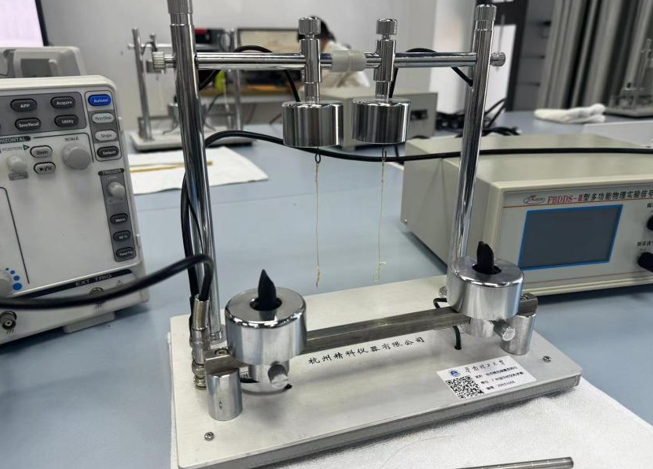
\includegraphics[clip,scale=0.5,trim={0 0 0 0}]{fig/fig1.png}
	                \label{figure.11}
	                \caption{FB2729A Dynamic Young's Modulus Experimental Instrument}
	             \end{minipage}
	             \begin{minipage}[t]{0.5\linewidth}
	                \centering
	                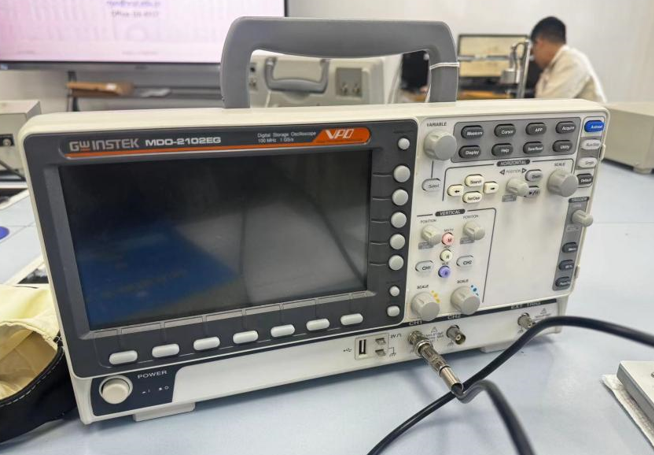
\includegraphics[clip,scale=0.5,trim={0 0 0 0}]{fig/fig2.png}
	                \label{figure.12}
	                \caption{dual-trace oscilloscope}
	             \end{minipage}   	  
	          \end{figure}    
    
	\begin{itemize}
	    \item \textbf{FB2729A Dynamic Young's Modulus Experimental Instrument:} Instrument used for measuring the dynamic Young's modulus of materials. The instrument features high precision and multifunctionality, suitable for materials mechanics experiments.
	
	    \item \textbf{Multifunctional Audio Signal Source:} Versatile audio signal source providing signals of various frequencies and amplitudes. It can be used for different types of experiments and testing.
	
	    \item \textbf{Dual-Trace Oscilloscope:} Two-channel oscilloscope used for observing and analyzing waveforms of electrical signals. It is applicable for measuring and analyzing voltage signals generated in experiments.
	
	    \item \textbf{Electronic Balance:} Precision electronic balance used for accurate measurement of the mass of objects. It is suitable for experiments and practical applications requiring high-precision mass measurements.
	
	    \item \textbf{Steel Ruler:} Tool for measuring length. In experiments, it can be used to measure the linear dimensions of various objects.
	
	    \item \textbf{Vernier Caliper:} Vernier caliper for measuring the length, width, and thickness of objects. It provides high-precision dimensional measurements.
	
	\end{itemize}
    
 \begin{figure}[H]
             \begin{minipage}[t]{0.5\linewidth}
                \centering
                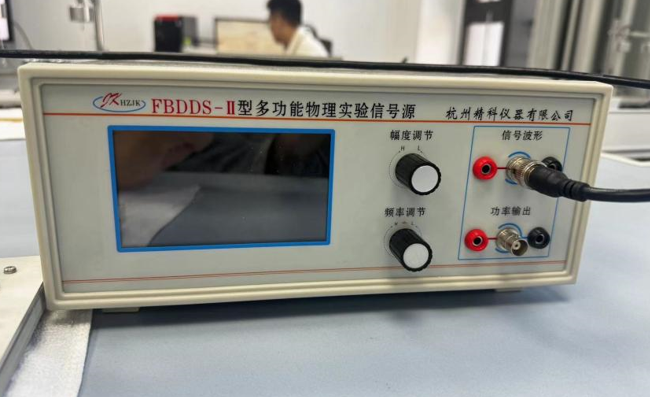
\includegraphics[clip,scale=0.5,trim={0 0 0 0}]{fig/fig3.png}
                \label{figure.11}
                \caption{multifunctional audio signal source}
             \end{minipage}
             \begin{minipage}[t]{0.5\linewidth}
                \centering
                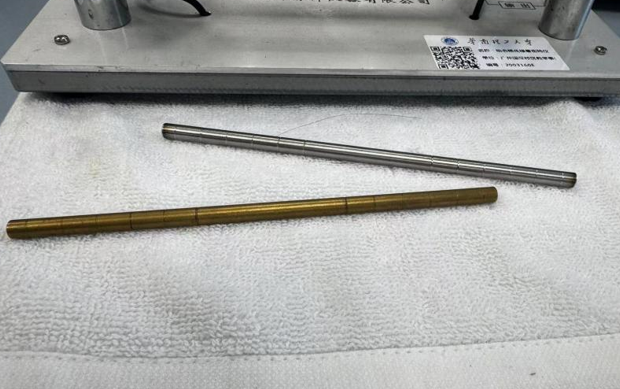
\includegraphics[clip,scale=0.5,trim={0 0 0 0}]{fig/fig4.png}
                \label{figure.12}
                \caption{solid materials}
             \end{minipage}   	  
          \end{figure}       
    
        
	\section{Experimental principles}   
    \subsection{Physical basis of Young's modulus measurements by the resonance method}
    The Young's modulus measurement by the resonance method is based on the theory of vibration analysis of free beams. According to the transverse vibration of the bar equation:
    
    \begin{eqnarray}
    \frac{\partial^{4} \mathrm{Y}}{\partial \mathrm{x}^{4}}+\frac{-\rho S}{E J} \cdot \frac{\partial^{2} \mathrm{Y}}{\partial \mathrm{t}^{2}}=0
    \end{eqnarray}
    
    Where:$Y$ is the vibrational displacement of the plasmonic element of the rod at $x$; $E$ is the Young's modulus of the rod; $S$ is the cross-sectional area of the rod $J$ is the rotational moment of inertia of the rod; $\rho$ is the density of the rod; $x$ is the positional coordinates of the plasmonic element; and $t$ is the time variable.
    
    The method of separated variables solves the equation of transverse vibration of the rod, so that $Y(x, t) = X(x)∙T(t)$, and substituting into equation yields:
    
    \begin{eqnarray}
    \frac{1}{X} \cdot \frac{\partial^{4} \mathrm{Y}}{\partial \mathrm{x}^{4}}=\frac{\rho S}{E J} \cdot \frac{1}{T} \frac{\partial^{2} \mathrm{Y}}{\partial \mathrm{t}^{2}}
    \end{eqnarray}
    
    It can be seen that both sides of the above equation are functions of $x$ and $t$, respectively, and that the equation can only be made to hold if both are equal to an arbitrary constant. Setting this constant to $K^4$ gives:
    
    \begin{eqnarray}
    \frac{\partial^{4} \mathrm{X}}{\partial \mathrm{x}^{4}}-\mathrm{K}^{4} \mathrm{X}=0 \\
    \frac{\partial^{2} \mathrm{~T}}{\partial \mathrm{t}^{2}}-\frac{\mathrm{K}^{4} E J}{\rho S} \cdot \mathrm{T}=0 
    \end{eqnarray}
    
    Solving these two linear ordinary differential equations yields the general solution:
    
    \begin{eqnarray}
    \mathrm{Y}(\mathrm{x}, \mathrm{t})=\left(\mathrm{A}_{1} \operatorname{chkx}+\mathrm{A}_{2} \operatorname{shkx}+\mathrm{B}_{1} \operatorname{coskx}+\mathrm{B}_{2} \operatorname{sinkx}\right) \cos (\mathrm{wt}+\varphi)
    \end{eqnarray}
    
    Which;
    
    \begin{eqnarray}
    w = (\frac{K^{4}EJ}{\rho S})^{\frac{1}{2}}
    \end{eqnarray}
    
    It is called the frequency equation. $A_1, A_2, B_1, B_2, \phi$ are the coefficients to be determined, which can be determined from the boundary conditions and the initial conditions.
    
    For a bar of length L with free ends, the boundary conditions are when the suspension line hangs near the nodes of the bar: The transverse force at the free end is zero, and the bending moment is also zero. That is
    
    \begin{eqnarray}
    \frac{\partial^{4} \mathrm{y}}{\partial \mathrm{x}^{3}}=0(\mathrm{x}=0) \quad \frac{\partial^{3} \mathrm{y}}{\partial \mathrm{x}^{3}}=0(\mathrm{x}=\mathrm{L}) \\
    \frac{\partial^{2} \mathrm{y}}{\partial \mathrm{x}^{2}}=0(\mathrm{x}=0) \quad \frac{\mathrm{K}^{4} \mathrm{y}}{\partial \mathrm{x}^{2}}=0(\mathrm{x}=\mathrm{L})
    \end{eqnarray}
    
    Substituting the boundary conditions into the generalized solution yields the transcendental equation:
    
    \begin{eqnarray}
    \operatorname{coskL} \cdot \operatorname{chkL}=1
    \end{eqnarray}
    
    The roots of the equation are obtained by numerical calculations, in order $kL = 0$, $4.7300$, $7.8532$, $10.9956$, $14. 137$, $17.27$, $20.420$ $\dots$ This number gradually converges to the value of the expression $kL=(n-1/2)\pi$.
    
    The first root $0$ above corresponds to the static value, and the second root is noted as $kL = 4.7300$, with which the resonant frequency is called the fundamental (or intrinsic) $frequency = 2$. According to equation, the Young's modulus of the specimen can be obtained as:
    
    \begin{eqnarray}
    \mathrm{E}=\frac{\omega^{2} \rho S}{\mathrm{~K}^{4} J}=\frac{\left(2 \pi f_{1}\right)^{2} \rho S}{\mathrm{~K}^{4} J}
    \end{eqnarray}
    
    For a circular rod with diameter $d$, length $L$, and mass $m$, its moment of inertia is $J = (Sd^2)/16$, density $\rho=4m/(\pi d^2 L)$, and $K_1L = 4.7300$. Substituting into the equation yields Young's modulus of the rod:
    
    \begin{eqnarray}
    \mathrm{E}=1.6067 \frac{L^3mf_{1}^2}{d^4}
    \end{eqnarray}
    
    From this, the Young's modulus of a rod can be measured as long as the resonant fundamental frequency of the rod can be measured.
    
   
   \subsection{Measurement of the resonant fundamental frequency of a specimen rod}
   The key to measuring Young's modulus using the resonance method lies in determining the resonance fundamental frequency of the sample rod. The principle of measuring Young's modulus using the resonance method is illustrated in Figure. The sinusoidal electrical signal, generated by the audio signal source with a continuously adjustable frequency, is converted into mechanical vibrations of the same frequency by the exciter. These mechanical vibrations are then transmitted to the sample rod through a suspension wire, which decouples the system. The sample rod undergoes forced transverse vibrations at its end where the suspension wire is attached. The vibrations of the sample rod are transmitted back to the transducer by another suspension wire, converting the mechanical vibrations back into electrical signals. These signals are then filtered and amplified by a frequency-selective amplifier before being displayed on an oscilloscope.
   
   \begin{figure}[H]
   	    	\centering
   	    	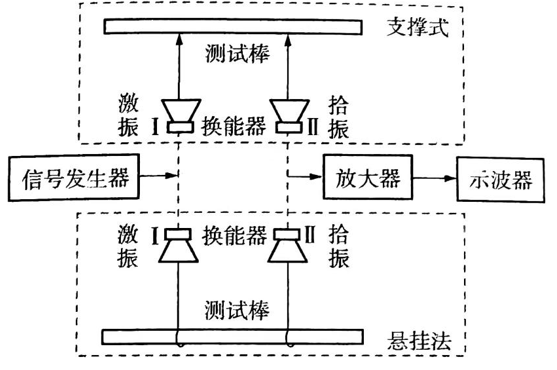
\includegraphics[clip,scale=1,trim={0 0 0 0}]{fig/fig5.png}
   	        \caption{Measurement of Young's modulus by resonance method}
   	        \label{figure.1}
       \end{figure}  
   
   When the frequency of the signal source does not match the natural frequency of the sample rod, the rod does not undergo resonance, resulting in minimal or almost no electrical signal waveform on the oscilloscope, or the waveform has a very small amplitude. However, when the frequency of the signal source equals the natural frequency of the sample rod, resonance occurs. At this point, the waveform amplitude on the oscilloscope suddenly increases, and the frequency displayed by the instrument corresponds to the resonance frequency of the sample rod under the specific suspension conditions.
   
   The transverse vibration nodes of the rod are related to the vibration order. Figure illustrates the vibration waveforms for $n = 1, 2, 3, 4$. From the $n=1$ waveform, it can be observed that the sample rod has two nodes during the fundamental frequency resonance, positioned at distances of $0.224L$ and $0.776L$ from one end, respectively. Theoretically, the suspension point should be chosen at one of these nodes to obtain the fundamental resonance frequency of the sample rod.
   
   \begin{figure}[H]
      	    	\centering
      	    	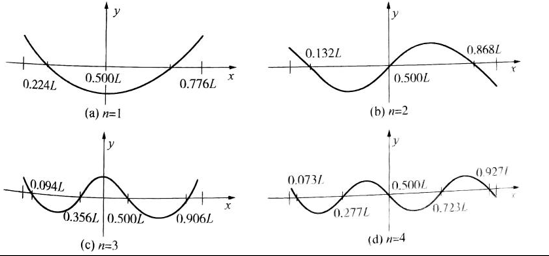
\includegraphics[clip,scale=1.1,trim={0 0 0 0}]{fig/fig6.png}
      	        \caption{The vibration waveforms for $n = 1, 2, 3, 4$}
      	        \label{figure.1}
          \end{figure}
   
   In the experiment, the detected resonance frequency varies with the position of the suspension point due to the damping effect of the suspension wire on the vibration of the sample rod. As the position of the suspension point changes, the detected resonance frequency also changes. Since the piezoelectric transducer picks up the acceleration resonance signal at the suspension point rather than the amplitude resonance signal, the detected resonance frequency increases with the distance from the suspension point to the node.
   
   Directly measuring the fundamental frequency resonance of the sample rod requires suspending the wire at the node. In the fundamental frequency vibration mode of the sample rod, there are two nodes, positioned at distances of $0.224L$ and $0.776L$ from one end. As the amplitude at the nodes is almost zero, making it challenging to excite and detect vibrations, an extrapolation measurement method is employed to determine the fundamental frequency resonance of the sample rod. The extrapolation method involves obtaining values beyond the range of measured data, which is generally difficult to measure. To determine this value, a graphical extrapolation method is used. This entails plotting a curve using the measured data, extending the curve according to the original pattern to the desired value range, and extracting the required values from the extended portion.
   
   It is important to note that the extrapolation method is only applicable when there are no sudden changes within the studied range; otherwise, it is not suitable.
   
   \begin{figure}[H]
      	    	\centering
      	    	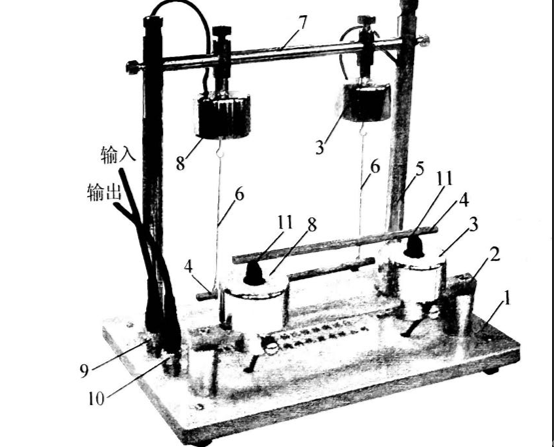
\includegraphics[clip,scale=1,trim={0 0 0 0}]{fig/fig7.png}
      	        \caption{Suspended and Supported Dynamic Young's Modulus Test Bench}
      	        \label{figure.1}
          \end{figure}
       
    The intrinsic frequency $f_{intrinsic}$ of the specimen bar and the fundamental resonance frequency $f_{resonance}$ are two different concepts, and the relationship between them is:
    
    \begin{eqnarray}
    f_{\text {intrinsic}}=f_{\text {resonance}} \sqrt{1+\frac{1}{4 Q^{2}}}
    \end{eqnarray}
    
    where $Q$ is the mechanical quality factor of the specimen bar. For the suspension method of measurement, the general $0$ value is greater than $50$, the fundamental frequency co-frequency and the intrinsic frequency compared to only $0.005\%$ lower, so in the experiment can be used to replace the group frequency with the fundamental frequency resonance frequency, with formula to calculate the Young's modulus.
   
      
               
	\section{Contents and Steps}

\begin{itemize}

    \item \textbf{Familiarize yourself with the structure and operating procedures:}
    \begin{itemize}
        \item Connect the dynamic Young's modulus tester.
        \item Power on the apparatus and allow a 10-minute preheating period.
    \end{itemize}

    \item \textbf{Measure sample parameters:}
    \begin{itemize}
        \item Measure length $(L)$, diameter $(d)$, and mass $(m)$ of the sample.
        \item Conduct five measurements for each parameter, recording data in Table.
        \item Calculate positions of two nodes on the sample rod ($0.224L $and $0.776L$) and mark them.
        \item Mark positions of suspension points on the sample rod for resonance frequency measurement.
    \end{itemize}

    \item \textbf{Set up suspension system:}
    \begin{itemize}
        \item Suspend the sample rod from two wires with attachment points at$ -30mm$ and $-30mm$.
        \item Adjust movable support on the crossbeam for perpendicular suspension wires.
        \item Ensure suspension wires are aligned horizontally.
        \item Check the installation meets requirements in a stationary state.
    \end{itemize}

    \item \textbf{Measure resonance frequency using suspension method:}
    \begin{itemize}
        \item Slowly adjust frequency knob to find resonance frequency.
        \item Fine-tune frequency knob for maximum amplitude on the oscilloscope, indicating resonant state.
        \item Record resonance frequency at this position.
        \item Change suspension points and support positions as required, recording data in Table.
    \end{itemize}

    \item \textbf{Support method:}
    \begin{itemize}
        \item Remove sample rod from suspension wires.
        \item Place it gently on the rubber support blade of the support-style exciter/pickup.
        \item Connect signal generator to testing platform and amplifier, and oscilloscope as described.
    \end{itemize}

    \item \textbf{Follow the remaining steps as in the suspension method.}

\end{itemize}
	
	\section{Data processing}
   \subsection{Experimental measurement data recording}
   Specimen bar1 length $L=160mm$; Specimen bar1 mass $m=0.035kg$; Specimen bar1 radius $d=6mm$; Specimen bar2 length $L=160mm$; Specimen bar2 mass $m=0.038kg$; Specimen bar1 radius $d=6mm$.
       
   \begin{table}[htbp]
       \centering
       \caption{Measurement of resonant frequency (Copper)}
       \begin{tabular}{cccccccc}
           \toprule
           \textbf{Position of Suspension Point} && \textbf{1} & \textbf{2} & \textbf{3} &\textbf{4} & \textbf{5} & \textbf{6} \\
           \midrule
                                            & 1 & 769.00 & 750.30 & 734.63 & / & 731.84 & 738.66 \\
                    \textbf{Resonant Frequency}& 2 & 769.66 & 748.56 & 733.56 & / & 731.76 &738.86\\
                              $f$ (Hz)       & 3 & 769.45 & 748.55 & 733.85 & / & 731.85 & 738.95\\
                                              &$\bar{f}$  & 769.37 & 749.14 &  734.01 &/ & 731.82 & 738.82 \\
           \bottomrule
       \end{tabular}
       \label{tab:resonant-frequencies}
   \end{table}
   
\begin{table}[htbp]
    \centering
     \caption{Measurement of resonant frequency (Steel)}
    \begin{tabular}{cccccccc}
        \toprule
        \textbf{Position of Suspension Point} && \textbf{1} & \textbf{2} & \textbf{3}  &\textbf{4} & \textbf{5} & \textbf{6} \\
        \midrule
                                           & 1 & 1049.16 & 1057.26 & 1062.96 & / & 1064.16 & 1061.16\\
         \textbf{Resonant Frequency}       & 2 & 1050.16 & 1056.06 & 1062.06 & / & 1063.56 & 1059.49\\
                $f$ (Hz)                   & 3 & 1050.76 & 1056.76 & 1062.46 & / & 1063.56 & 1060.66\\
                                           &$\bar{f}$  & 1050.03 & 1056.69 & 1062.49 & / & 1063.76 & 1060.44\\
        \bottomrule
    \end{tabular}

    \label{tab:updated-resonant-frequencies}
\end{table}
  
   
   \subsection{Intrinsic frequency calculation}
   Now it is necessary to fit the curve by using the data 1, 2, 3, 5 and 6 times and in this way obtain the resonance frequency of the material as follows:
   
   Measurement of resonant frequency (Copper):
   
   	 \begin{figure}[H]
         \begin{minipage}[t]{0.33\linewidth}
            \centering
            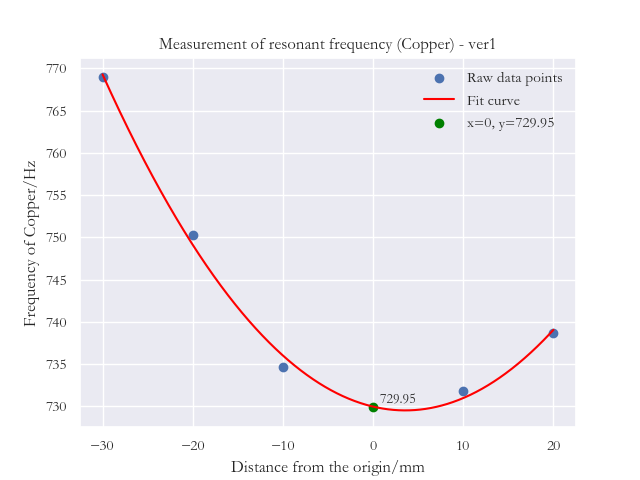
\includegraphics[clip,scale=0.35,trim={0 0 0 0}]{fig/fig8.png}
            \label{figure.11}
         \end{minipage}
         \begin{minipage}[t]{0.33\linewidth}
            \centering
            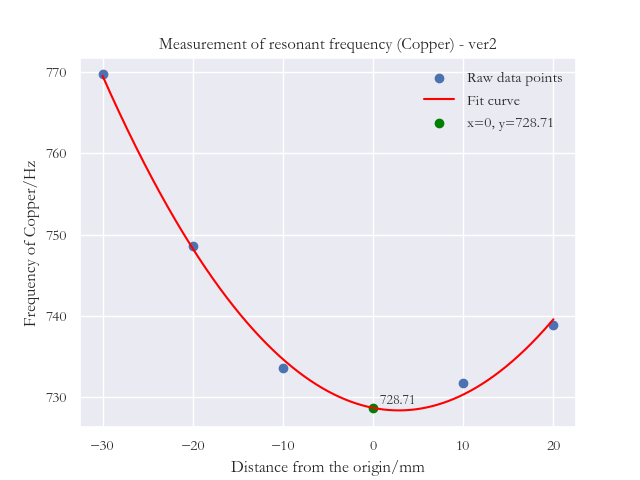
\includegraphics[clip,scale=0.35,trim={0 0 0 0}]{fig/fig9.png}
            \label{figure.12}
         \end{minipage}  
         \begin{minipage}[t]{0.33\linewidth}
         \centering
         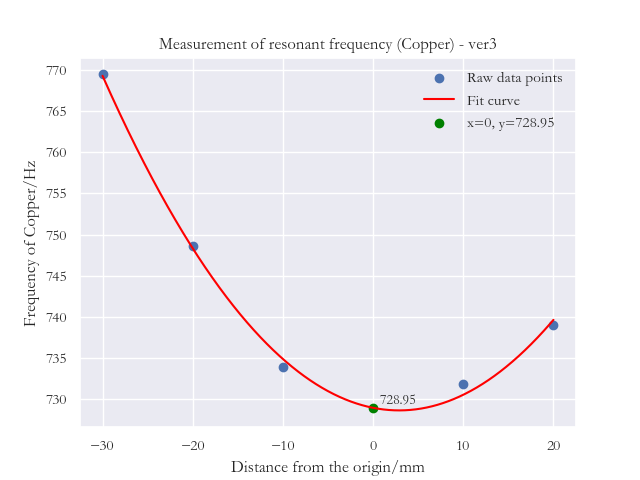
\includegraphics[clip,scale=0.35,trim={0 0 0 0}]{fig/fig10.png}
         \label{figure.12}
      \end{minipage} 
     \caption{Measurement of resonant frequency (Copper)}	  
      \end{figure}   
   	          
   	 We obtained the following resonant frequencies for the three data sets:
   	 
   	 \begin{eqnarray}
   	 f_1 = 729.95 Hz \qquad f_2 = 728.71 Hz \qquad f_3 = 728.95 Hz
   	 \end{eqnarray}
   	 
   	 So the mean and variance are obtained as follows:
   	 \begin{eqnarray}
   	 \bar{f} = 729.20 \qquad \sigma_f = 0.284
   	 \end{eqnarray}
   	 
   	 So the resonant frequency of Copper is :
   	 
   	 \begin{eqnarray}
   	 f = 729.20 \pm 0.284 Hz
   	 \end{eqnarray}
   	 
   	 Measurement of resonant frequency (Stool):
   	 \begin{figure}[H]
         \begin{minipage}[t]{0.33\linewidth}
            \centering
            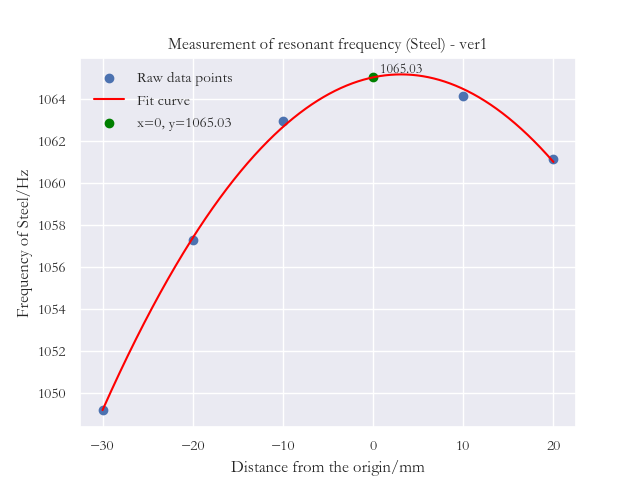
\includegraphics[clip,scale=0.35,trim={0 0 0 0}]{fig/fig11.png}
            \label{figure.11}
         \end{minipage}
         \begin{minipage}[t]{0.33\linewidth}
            \centering
            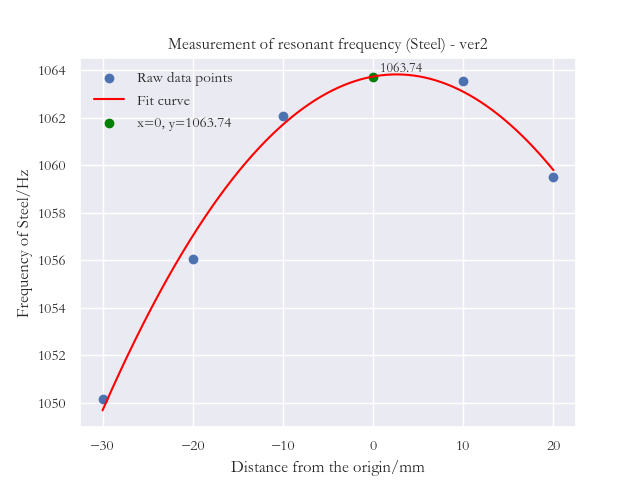
\includegraphics[clip,scale=0.35,trim={0 0 0 0}]{fig/fig12.png}
            \label{figure.12}
         \end{minipage}  
         \begin{minipage}[t]{0.33\linewidth}
         \centering
         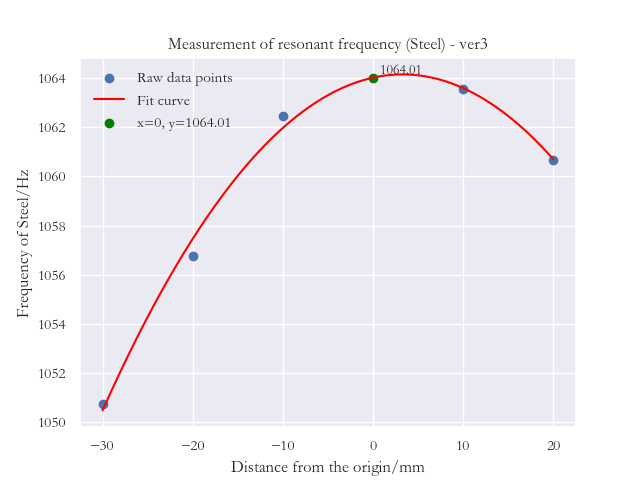
\includegraphics[clip,scale=0.35,trim={0 0 0 0}]{fig/fig13.png}
         \label{figure.12}
      \end{minipage} 
     \caption{Measurement of resonant frequency (Stool)}	  
      \end{figure}  
      
       We obtained the following resonant frequencies for the three data sets:
         	 
         	 \begin{eqnarray}
         	 f_1 = 1065.03 Hz \qquad f_2 = 1063.74 Hz \qquad f_3 = 1064.01 Hz
         	 \end{eqnarray}
         	 
         	 So the mean and variance are obtained as follows:
         	 \begin{eqnarray}
         	 \bar{f} = 1064.26 \qquad \sigma_f = 0.309
         	 \end{eqnarray}
         	 
         	 So the resonant frequency of Copper is :
         	 
         	 \begin{eqnarray}
         	 f = 1064.26 \pm 0.309 Hz
         	 \end{eqnarray}    	 
   	 
   	 
   	 
   
   \subsection{Young's modulus calculation}
   
  The Young's modulus can be calculated from the formula as follows:
  
  \begin{eqnarray}
  E_{Copper} = 1.6067 \frac{L^3mf_{1}^2}{d^4} = 9.4504 \times 10^10 N/m^2\\
  E_{Stool} = 1.6067 \frac{L^3mf_{1}^2}{d^4} = 2.1856 \times 10^11 N/m^2
  \end{eqnarray}
  

\section{Conclusion and analysis}
\subsection{Conclusion}
In conclusion, the dynamic Young's modulus experiment involved the precise measurement of resonance frequencies using the resonance method and the support method. By supporting the sample rod and adjusting various parameters, including support points and support positions, resonance frequencies were determined under different conditions. The data collected allowed us to calculate the fundamental frequency of the sample rod, taking into account the positions of nodes and support points. The extrapolation method was employed to obtain accurate measurements, overcoming challenges posed by the amplitude at nodal points. This experiment not only enhanced our understanding of Young's modulus measurement principles but also underscored the importance of careful experimental setup and data interpretation.
The final result is obtained as follows:
  \begin{eqnarray}
  E_{Copper} = 1.6067 \frac{L^3mf_{1}^2}{d^4} = 9.4504 \times 10^10 N/m^2\\
  E_{Stool} = 1.6067 \frac{L^3mf_{1}^2}{d^4} = 2.1856 \times 10^11 N/m^2
  \end{eqnarray}

\subsection{Error analysis}
\begin{itemize}

    \item \textbf{Measurement Errors:}
    \begin{itemize}
        \item \textbf{Instrumental Errors:} Inaccuracies in the dynamic Young's modulus tester, oscilloscope, signal generator, or other equipment can introduce systematic errors.
        \item \textbf{Human Errors:} Errors introduced during the measurement process, such as misreading values on instruments, imprecise marking of positions, or inconsistent adjustment of equipment.
    \end{itemize}

    \item \textbf{Systematic Errors:}
    \begin{itemize}
        \item \textbf{Misalignment of Equipment:} If the sample rod, suspension wires, or support system are not perfectly aligned, it can lead to deviations in the resonance frequency measurements.
        \item \textbf{Temperature Fluctuations:} Changes in temperature during the experiment can affect the material properties and introduce systematic errors.
    \end{itemize}

    \item \textbf{Random Errors:}
    \begin{itemize}
        \item \textbf{Reading Variability:} Small variations in reading the resonance frequency on the oscilloscope or other instruments can contribute to random errors.
        \item \textbf{Vibrational Interference:} External vibrations or disturbances in the environment may introduce random errors in the measurements.
    \end{itemize}

    \item \textbf{Data Analysis Errors:}
    \begin{itemize}
        \item \textbf{Interpolation Errors:} Determining the exact position of resonance nodes on the sample rod for interpolation introduces uncertainties.
        \item \textbf{Calculation Errors:} Errors in calculating average values or other derived quantities from the collected data.
    \end{itemize}

    \item \textbf{Mitigation Strategies:}
    \begin{itemize}
        \item \textbf{Calibration:} Regular calibration of instruments to minimize instrumental errors.
        \item \textbf{Careful Setup:} Ensuring precise alignment and setup of experimental apparatus.
        \item \textbf{Environmental Control:} Minimizing temperature fluctuations and isolating the experiment from external vibrations.
        \item \textbf{Repeat Measurements:} Conducting multiple trials and averaging results to reduce random errors.
    \end{itemize}

\end{itemize}


\begin{appendix}
 \section{Experimental data recording graph} 
     	\begin{figure}[H]
     	    	\centering
     	    	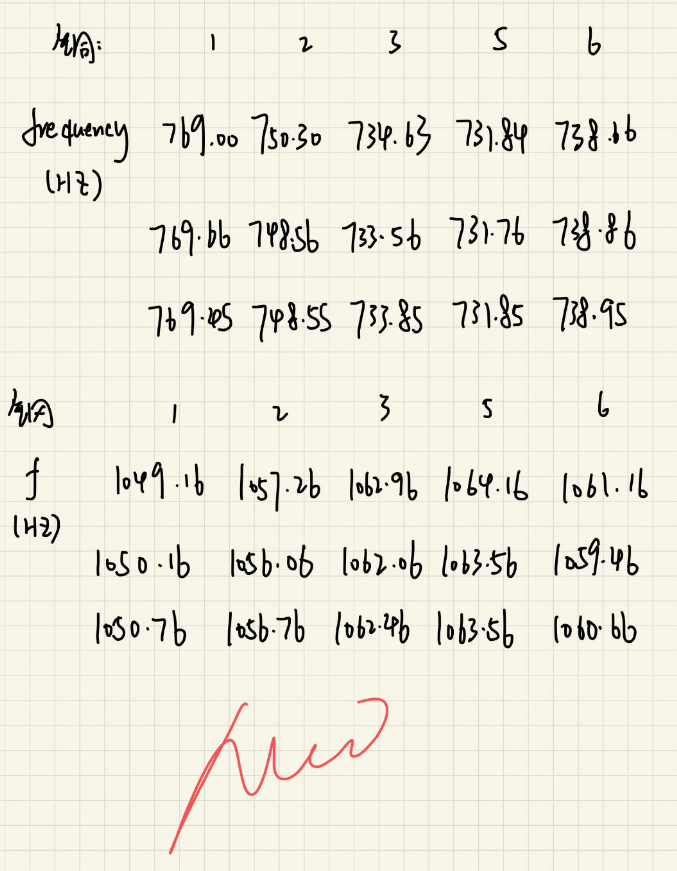
\includegraphics[clip,scale=0.8,trim={0 0 0 0}]{fig/fig14.png}
     	        \caption{Experimental data recording graph}
     	        \label{figure.19}
         \end{figure} 
 \end{appendix}        
\end{document}  